\documentclass[journal, a4paper]{IEEEtran}
\usepackage{graphicx}
\usepackage{url} 
\usepackage{amsmath}
\usepackage{subcaption}
\begin{document}

% Define document title and author
	\title{Homework 2: Part-of-Speech Tagging with HMMs and CRFs}
	\author{Guangyu Lin, EID: gl8429
}
	\markboth{CS 388 Natural Language Processing - University of Texas at Austin}{}
	\maketitle

% Write abstract here
\begin{abstract}
	The short report is intended to present homework 2, Part-of-Speech Tagging with HMMs and CRFs. Part-of-Speech tagging is the process of assigning some tags or syntactic class maker to each tokens in a sequence of natural language. The author uses Hidden Markov Model(HMM) and Conditional Random Field(CRF) to train and test on the datasets of Airline Booking Conversations and Wall Street Journal. The author also adds and compares some extra features, and changes the iterations for CRF. Moreover, the author try backward models as homework 1 and  find a trade off between HMM and CRF, as HMM is faster and CRF has more accuracy.
\end{abstract}

% Each section begins with a \section{title} command
\section{Introduction}
\subsection{Hidden Markov Model}
A hidden Markov model can be considered a generalization of a mixture model where the latent variables, which control the mixture component to be selected for each observation, are related through a Markov process rather than independent of each other.~\cite{HMM01} Therefore, we assume there is an underlying set of hidden states in which Part-of-Speech Tagging and there is probabilistic transitions between states over time.~\cite{SLIDE03} HMM is very useful to classify and order sequences, to tag each token in a sequence with a label and to train models to fit empirical training data. It models the full joint distribution of labels and observations to generate the most likely state sequence. However, the characteristic of HMM doesn't benefit the sequence labelling task.

\subsection{Conditional Random Field}
Conditional Random Field(CRF) is a discriminative model.~\cite{CRF01} As CRFs only model the conditional distribution $P(Y|X)$ and they are specifically designed ant trained to maximise performance of sequence labelling, it has much better performance than generative models when given a reasonable amount of training data. CRFs also easily allow adding additional token features without making additional independence assumptions. Therefore, we call CRFs a state-of-the-art method for sequence labelling.

This report explores a modification of a HMM and a CRF~\cite{MALLET} and experimentally test it on English dataset, which includes Airline Booking Conversations(ATIS) and Wall Street Journal(WSJ).  We modify the original model to measure accuracy for specially for out-of-vocabulary(OOV) items. We also calculate the specific OOV accuracy and OOV percentage of total test tokens. Then, we draw several tables and several figures of comparative results and states a discussion about trade off between different models.
	
The report is organized as following, the algorithms of calculating OOV accuracy and adding extra features are described briefly in Section~\ref{algorithm}. The results table and figure is provided in Section~\ref{result}. We discuss our results in Section~\ref{discuss}. And Section~\ref{conclude} is the conclusion of the report.

% Main Part
\section{Algorithms}\label{algorithm}
\vspace{3mm}
We calculate $Accucary_{oov}$ on OOV items in the held-out test data. Then we derived from the following formula:
\[
  Accucary_{oov} = \frac{C_({correct oov})}{C_{oov}}
\]
As ATIS is a fairly small corpus and should run fairly quickly. We add a random-seed to produce different train/test splits and average results of 10 times. WSJ dataset is much larger. HMM can be trained and tested quickly using dynamic programming, but CRF lasts for such a long time. So for WSJ we train section 00 and test on section 01 first and then we try a larger corpus, which are section 00 and 01, and test on section section10 and 11. Iterations changes are compared for CRF. Moreover, we also add some features to our POS-tagging, which are:\\
\indent[1] {\bf ING} $\rightarrow$ Progressive tense \\
\indent[2] {\bf S} $\rightarrow$ Plural \\
\indent[3] {\bf PAST} $\rightarrow$ Past tense \\
\indent[4] {\bf SHORT} $\rightarrow$ Less than four characters \\
\indent[5] {\bf CAPS} $\rightarrow$ Starts with a capital letter\\ 
As we find an improvement of backward during the previous homework, so I also train and test by reversing the sentences. Meanwhile, we also record the runtime and the overall training accuracy and test accuracy during each test.
%\vspace{3mm}

\section{Experiment Results}\label{result}

We train and test ATIS datasets with a ratio of 8:2 ten times and we train Section 00 in WSJ and test Section 01 in WSJ. Table~\ref{tab:1} is the results of ATIS and Table~\ref{tab:2} is the results of WSJ. In the table, $CRF_{m,n}$ is the result of CRF after adding feature [m] and [n] and $CRF_{1-5}$ is the result of CRF after adding five features.  $CRF_{L}$ and $HMM_{L}$ represents larger corpus for CRF and HMM(two sections). The results include overall accuracy of training and test, specific OOV accuracy, OOV percentage(OOV \%) of total test tokens and total time.
	\begin{table}[!hbt]
		\begin{center}
		% Title of the table
		\caption{Dataset: ATIS - Forward}
		\label{tab:1}
		\begin{tabular}{|c|c|c|c|c|c|}
			\hline
			Model & HMM & CRF & $CRF_{1,2}$ & $CRF_{4,5}$ &$CRF_{1-5}$\\ \hline
			 Training Acc & 0.890  & 0.999 & 0.999 & 0.999 & 0.999\\ \hline
			 Test Acc  & 0.861 &  0.926 & 0.932 & 0.938 & 0.936\\ \hline
			OOV Acc & 0.191 & 0.282 & 0.311 & 0.328 & 0.433\\ \hline
			OOV \% & 0.036 & 0.036 & 0.036 & 0.036 & 0.036\\\hline
			 Total Time & 3.032 & 53.572 & 57.534 & 54.308 & 53.469\\ 
			 \hline
		\end{tabular}
		\end{center}
		\vspace{-5mm}
	\end{table}

	\begin{table}[!hbt]
		\begin{center}
		% Title of the table
		\caption{Dataset: WSJ - Forward}
		\label{tab:2}
		\begin{tabular}{|c|c|c|c|c|c|}
			\hline
			Model & HMM & CRF & $CRF_{1-5}$ & $HMM_{L}$ & $CRF_{L}$\\ \hline
			 Training Acc & 0.862  & 0.986 & 0.992 & 0.887 & 0.994 \\ \hline
			 Test Acc  & 0.785 &  0.794 & 0.873 & 0.833 &0.849\\ \hline
			OOV Acc & 0.379 & 0.476 & 0.679 & 0.409 &0.517\\ \hline
			OOV \% & 0.153 & 0.153 & 0.153 & 0.109 & 0.109\\\hline
			 Total Time & 62.918 & 3810.47 & 3349.664 & 288.68 &15232.6 \\ 
			 \hline
		\end{tabular}
		\end{center}
		\vspace{-5mm}
	\end{table}
	
	\begin{table}[!hbt]
		\begin{center}
		% Title of the table
		\caption{Dataset: ATIS - Backward}
		\label{tab:3}
		\begin{tabular}{|c|c|c|c|c|c|}
			\hline
			Model & HMM & CRF & $CRF_{1,2}$ & $CRF_{4,5}$ & $CRF_{1-5}$\\ \hline
			 Training Acc & 0.902 & 0.998 & 0.999 & 0.999 & 0.999 \\ \hline
			 Test Acc  & 0.875 &  0.928 & 0.934 & 0.931 & 0.943\\ \hline
			OOV Acc & 0.231 & 0.293 & 0.241 & 0.367 & 0.449 \\ \hline
				OOV \% & 0.030 & 0.030 & 0.030 & 0.030 & 0.030\\\hline
			 Total Time & 4.052 & 67.102 & 66.421 & 64.510 & 64.948  \\ 
			 \hline
		\end{tabular}
		\end{center}
		\vspace{-5mm}
	\end{table}
	
	\begin{table}[!hbt]
		\begin{center}
		% Title of the table
		\caption{Dataset: WSJ - Backward}
		\label{tab:4}
		\begin{tabular}{|c|c|c|c|c|c|}
			\hline
			Model & HMM & CRF & $CRF_{1-5}$ & $HMM_{L}$ & $CRF_{L}$\\ \hline
			 Training Acc & 0.863 & 0.996 & 0.993 & 0.889 & 0.996 \\ \hline
			 Test Acc  & 0.785 & 0.811 & 0.879 & 0.833 & 0.854\\ \hline
			OOV Acc & 0.383 & 0.479 & 0.658 & 0.409 & 0.519\\ \hline
			OOV \% & 0.153 & 0.153 & 0.153 & 0.109 & 0.109\\\hline
			 Total Time & 46.924 & 4068.75 & 2789.891 & 220.64 & 20605.6 \\ 
			 \hline
		\end{tabular}
		\end{center}
		\vspace{-5mm}
	\end{table}

\section{Discussion}\label{discuss}
For the overall test accuracy, CRF beats HMM each time not only in constraint corpus(ATIS), but also in diverse corpus(WSJ). Though the performance is not very distinctive, we can learn the difference between generative model and discriminative model clearly. From the experimental results, we find that discriminative methods(CRF) are usually more accurate since they are trained for a specific performance tasks, which is also the reason that CRFs almost reach 100\% for the training accuracy.  We could only say that the training accuracy by HMM seems good, but not a little competitive with CRFs'.

As we see OOV percentage is very small in a constraint corpus(ATIS) and OOV is almost 10\%-15\% for a diverse corpus. For the test accuracy among only OO items, it satisfies our expectation. CRF beats HMM each time again! The theory support is that HMM will struggle when it comes across with some unknown token because HMM need to calculate the join distribution. Then we can reach the conclusion that CRF performs better for speech tasks.

However, even in constraint corpus, the running time of CRF is more than 15 times of the running time of HMM. Training time of CRF increases a lot in diverse corpus, which are more than 60 times of the training time of HMM. Obviously, HMM calculate by dynamic programming and it reaches convergence within several iterations. But CRF has to do complex optimisations. HMM will not be influenced by increasing iterations because it converges earlier. However, for CRF when we increase the iterations as 500, 600, 750, 900, 1000, it increase as 0.259-0.353 .Though we increase the iterations for CRF will improve the accuracy, we should understand there is a trade-off with time cost.

Adding extra orthographic features to data really helps to increase accuracy, though we mark some false features(Past tense, Plural and Progressive tense). Comparing with no extra features CRF, the overall accuracy of train and test almost the same, but OOV accuracy improves a lot. The reason is the a few more extra features could help us gain more information while training the model. But the running time doesn't increase a lot for our experimental corpus. For ATIS, we add different two extra features, then add all five extra features. We find that OOV accuracy improves a lot, which is from 0.282 to 0.433, though they have a similar performance on test accuracy(0.926 and 0.936). We also compare two different features {\bf ING + S} and {\bf SHORT + CAPS}. The results shows that {\bf SHORT + CAPS} performances better than the other one. I guess false markers of plural and progressive tense is the reason.

One extension is to train in larger corpus(two sections) of WSJ by CRF and HMM. We find both performance improve a little when on larger corpus, however CRF costs times of previous running time. And OOV accuracy improves but not as significant as we expect. We should balance the time and accuracy based on our application.

Another extension is to try backward model as homework 1. As HMM is directional and CRF is in-directional, we expect to see difference between Forward HMM and Backward HMM and no difference between Forward CRF and Backward CRF. Unfortunately, we find the difference between two directional HMM and the difference between two directional CRF could not tell us this kind of character, which may be caused by the left sentences boundaries. 

\begin{figure}
        \begin{subfigure}[b]{0.24\textwidth}
                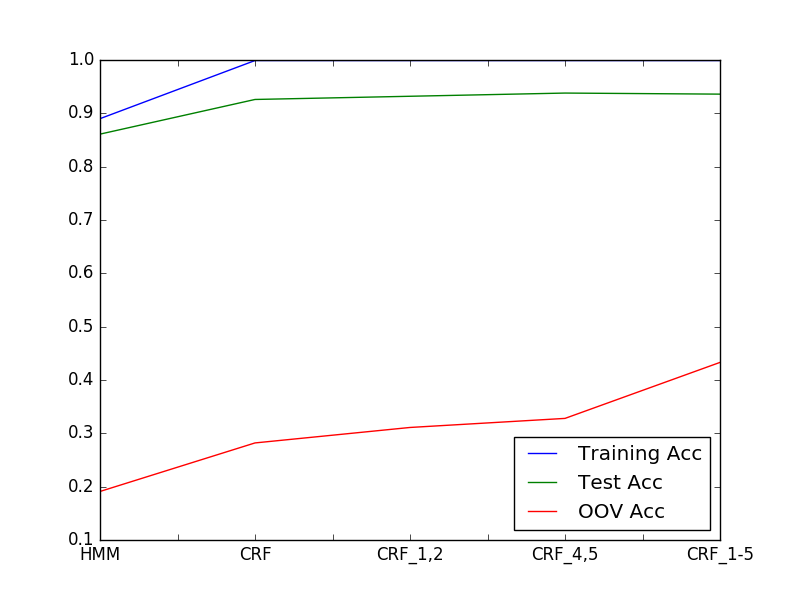
\includegraphics[width=\linewidth]{atis}
                \caption{Forward Model of ATIS}
                \label{fig:gull}
        \end{subfigure}%
        \hspace{\fill}
        \begin{subfigure}[b]{0.24\textwidth}
                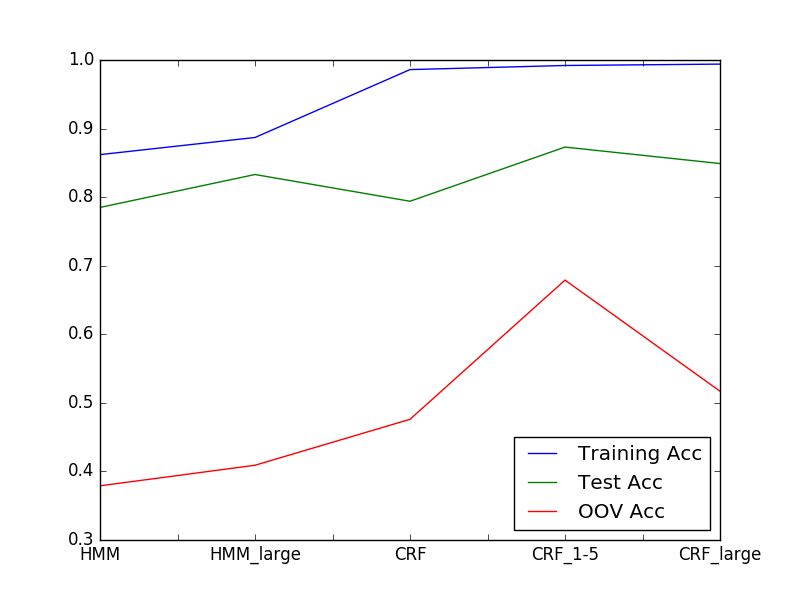
\includegraphics[width=\linewidth]{wsj}
                \caption{Forward Model of WSJ}
                \label{fig:gull2}
        \end{subfigure}%
        \hspace{\fill}
        \begin{subfigure}[b]{0.24\textwidth}
                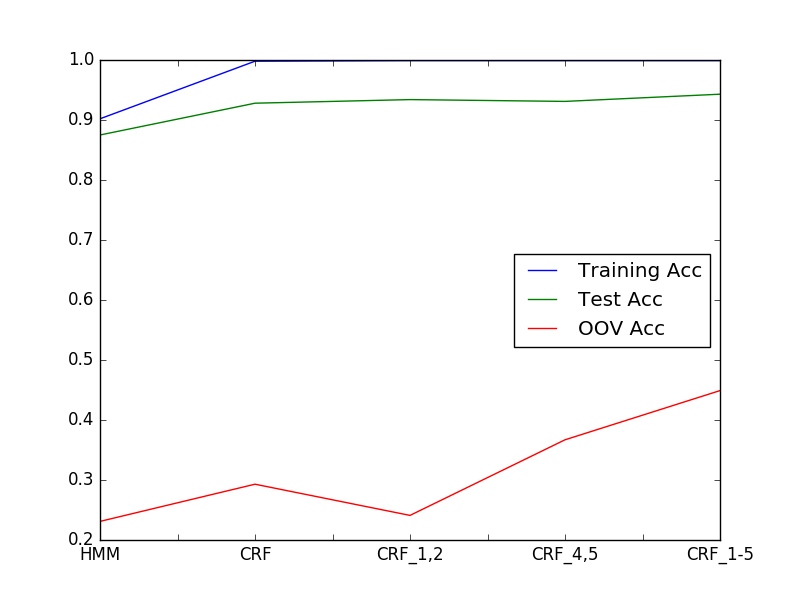
\includegraphics[width=\linewidth]{atisB}
                \caption{Backward Model of ATIS}
                \label{fig:tiger}
        \end{subfigure}%
        \hspace{\fill}
        \begin{subfigure}[b]{0.24\textwidth}
                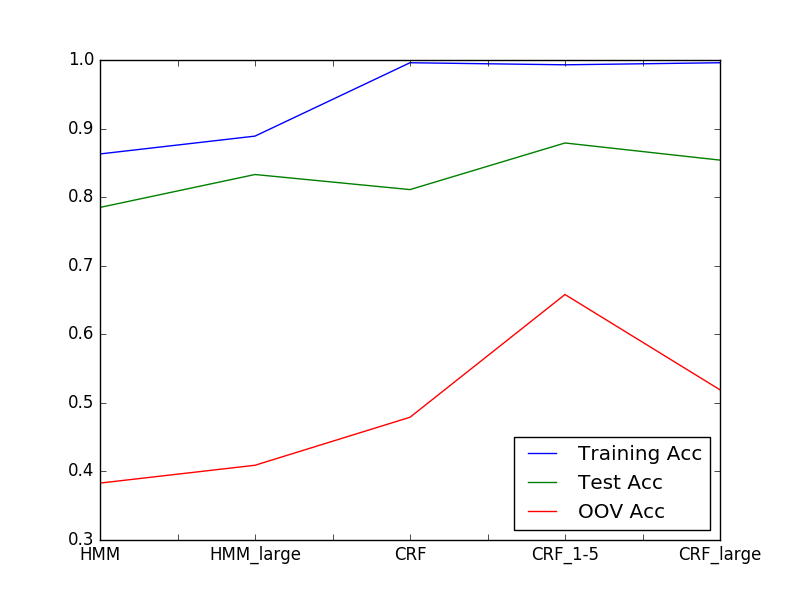
\includegraphics[width=\linewidth]{wsjB}
                \caption{Backward Model of WSJ}
                \label{fig:mouse}
        \end{subfigure}
        \caption{$CRF_{1,2}$ indicates adding features of ING + S, $CRF_{4,5}$ indicates adding features of SHORT + CAPS, $CRF_{1-5}$ indicates adding all five features, $CRF_{L}$ indicates larger corpus, $HMM_{L}$ indicates larger corpus}\label{fig:animals}
\vspace{-2mm}
\end{figure}


\section{Conclusion}\label{conclude}
	In this report, we talked about two different standard probabilistic sequence models, which are HMM and CRF. We train and test our models in a constraint corpus and a diverse corpus. We also add some features and compare the influence of different features for CRF. We also change iterations for CRF. Each time we analyse overall accuracy, OOV accuracy and training time among HMM and different kinds of CRFs.
	
% Now we need a bibliography:

% Your document ends here!
\end{document}